\section{Testing}
\label{sect:testing}

	As a distributed topology in a Big-Data environment could be a complex structure, testing is (as always) no marginal problem. In our Storm based scenario, we have Spouts that are emitting the initial input into the topology, Bolts that are executing operations on that input in one or several chains of neighbouring Bolts and we have the topology that combines Spouts and Bolt chains with each other to form a structure, which is able to solve a specific Big-Data analytics problem. 
	In such a scenario, it is not easy to find and solve problems and errors, as monitoring is only in place for the whole topology and not for each individual element. Additionally, a Storm topology is only debuggable at runtime, which makes it quite hard to find bugs or \textit{at least just realize that the topology is not working as expected} for large setups. 
	To find problems and errors in such a setup several points of view are needed to be addressed in order to find the source of a problem faster and more reliable as it would usually be the case.
	
\subsection{Test-Suite Approach}
\label{sect:TestSuiteApproach}
	In order to cope with the challenges of testing in complex and distributed Storm environments, we developed our own Test-Suite, which focuses on three different levels that may contain, combined with each other, the most common problem sources in an instance of one of our CIT-Storm topologies. The three different problem levels that we considered of importance were the following ones, sorted by abstraction level in the topology:
	
	\begin{description}
	 \descriptor{Operator-Tests}
		Are describing the validity of a specific user defined function that is caring about the input tuple execution inside a Bolt. For a well defined testing setup, each Bolt inside the testing topology should have an Operator- \& a Bolt-Test (described beneath) to fully assure that the respective Bolt is behaving as expected \textit{without any outside influences}, namely predecessor Bolts that are sending unexpected input to this Bolt. An Operator-Test is thus using pre-defined tuple input and checks if the asserted output of the operator to be tested is matching with the factual output.
		\begin{center}
			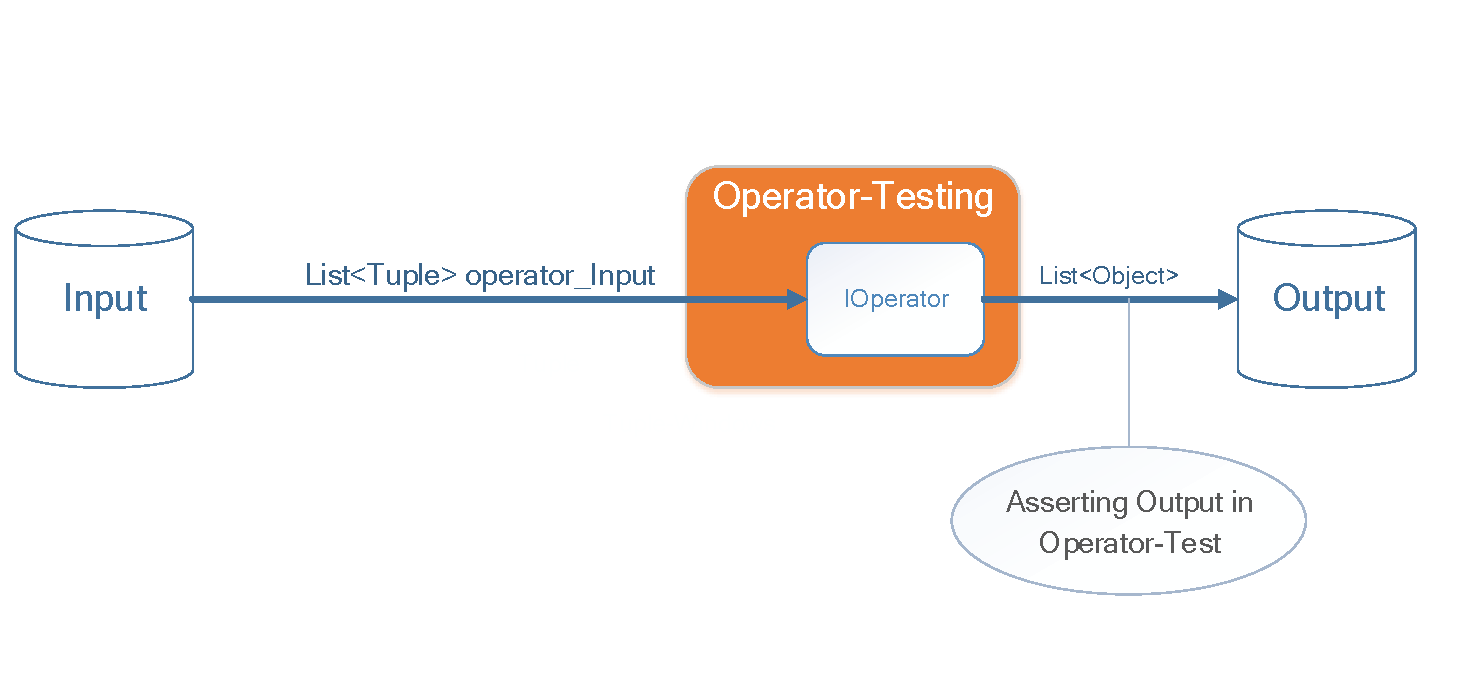
\includegraphics[width=0.4\textwidth]{./images/09_testing/OperatorTest.pdf}
		\end{center}

		
	 \descriptor{Bolt-Tests}
		Are combining Operator-Tests with additional Window-Handling, as needed to build streaming input execution. In our CIT-Storm implementation (as defined in \ref{sect:udfBolt}), we are using \textit{Time-} or \textit{Count-Windows} to wait a specific time or for a specific amount of input tuples, until the execution of those input tuples will be passed to the Operator. \\
		In perspective if this Testing-Suite, the Operator-Test (which was already successfully executed before) is only returning the correctness of a given input, relative to an asserted output, whereas a Bolt-Test includes testing with focus on the used window and its output after a \texttt{window.flush()}. The Bolt-Test will only be successful when a window returns the expected tuples after a given time and the Operator will correctly handle this input.
		\begin{center}
			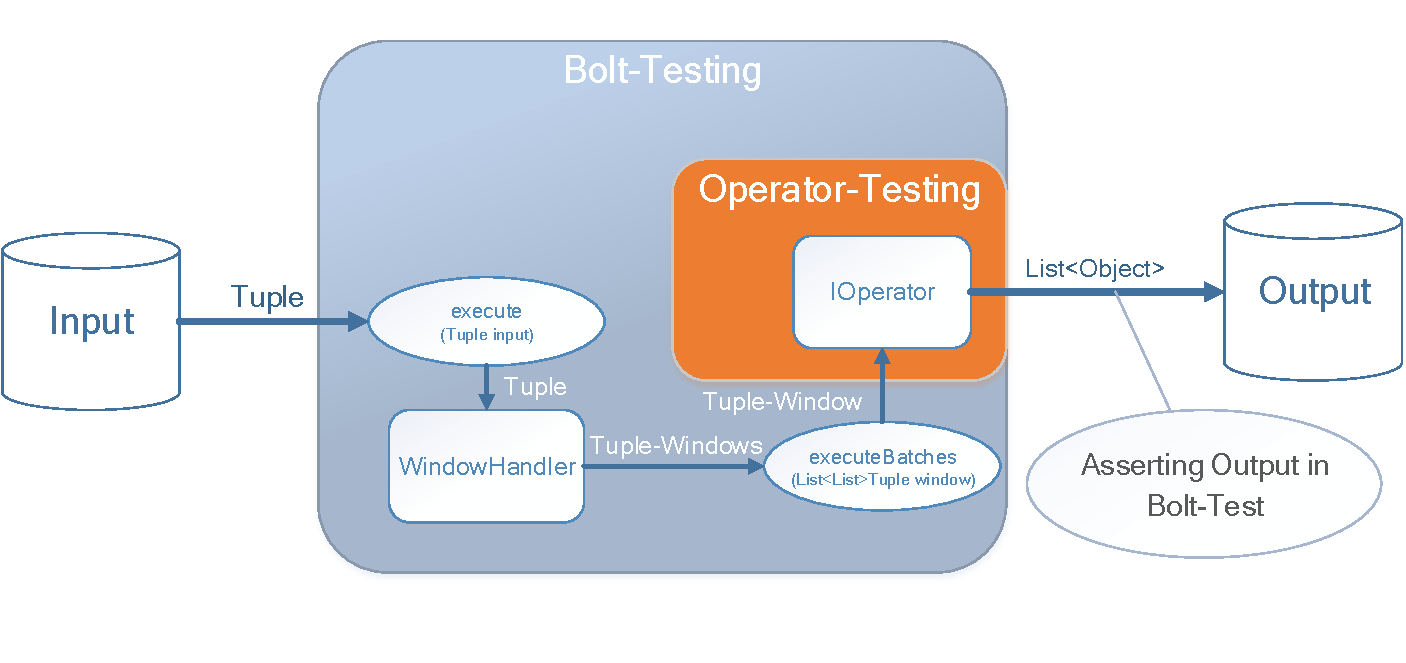
\includegraphics[width=0.4\textwidth]{./images/09_testing/BoltTest.pdf}
		\end{center}
	 
	 \descriptor{Topology-Tests}
		In order to test the topology as a whole, the Test-Suite provides a test skeleton named \texttt{TopologyTest}. A specific TopologyTest-Scenario is inherited by this class and allows the test-designer to test \textit{chains of Bolts with a Spout as source} in one run. Of course, this is not handling the complexity that Storm could cope with in its topologies, but as the Test-Suite is running outside a Storm environment (more on the implementation details may be found in the upcoming section \ref{sect:TestSuiteRealization}), it would be a likewise complex (and error-prone) task to completely simulate every aspect of Storm.\\
		The Topology-Test however does focus on linear topologies, which is describing most of the regular use-cases inside a Big-Data scenario. Even if the real Storm topology would use different Stream-Groupings (described in \ref{sect:StreamGroupings} on page \pageref{sect:StreamGroupings}), the shuffled topology input could mostly be baked onto a linear topology. \\
		In order to set up a TopologyTest, import each Bolt from the topology to be tested into the test-class's \texttt{defineTopologySetup()} and add the respective Bolt in a \texttt{BoltTestConfig} in the order you want them to be placed in the testing chain. Each \texttt{BoltTestConfig} is carrying the respective \texttt{UDFBolt}, a Bolt-TestName, a timeout per tuple input (needed for \texttt{TimeWindows}) and an assertedOutput with it, in order to fully define a TopologyTest. The test run is then defined as an execution of different Bolt-Tests, initialized by the different \texttt{BoltTestConfigs}. Each Bolt-Test receives the output of the predecessing Bolt-Test as its own input. A Topology-Test could thus only succeed, if each Bolt-Test (and the Operator-Tests inside it) succeeds and on top of that, if the final output matches with the final asserted output of the topology, respective to the initial input.
		\begin{center}
			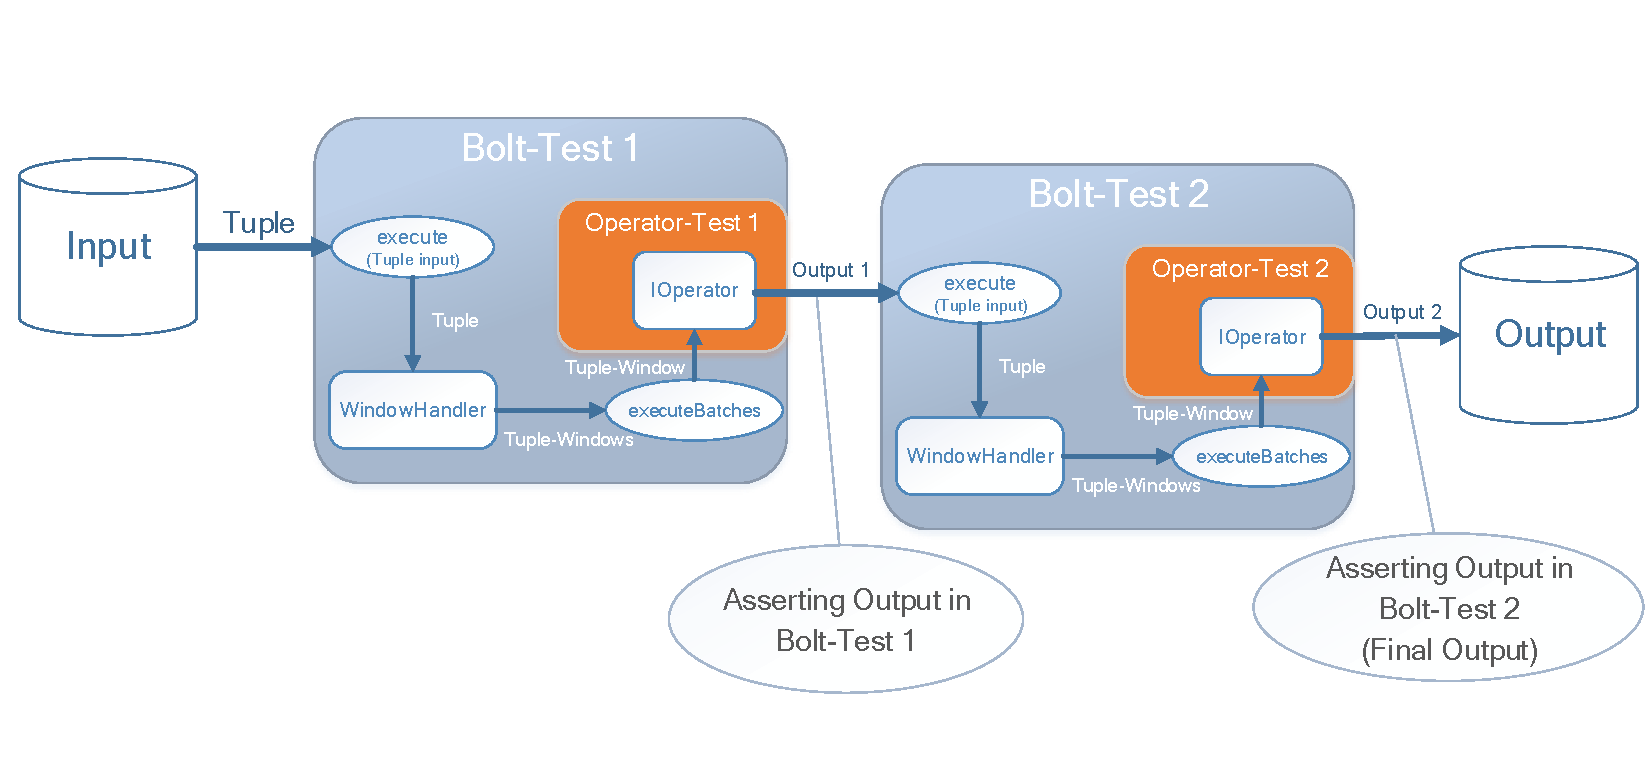
\includegraphics[width=0.4\textwidth]{./images/09_testing/TopologyTest.pdf}
		\end{center}
		
	\end{description}

\subsection{Test-Suite Realization}
\label{sect:TestSuiteRealization}
	The Test-Suite is independent from Storm, as the Bolt- and Operator-logic should be tested and not the Storm framework itself. Additionally, Storm defines some data types (the \texttt{Tuple}-class is the most famous example), which could not be easily constructed by themselves, even though a constructor would be needed for sufficient testing. This was another selection criteria to choose Mockito as the mockup base for our Class-Mocks - more about Mockito is described in section \ref{sect:Mockito}. \\
	The most interesting classes for a test-designer in the Test-Suite are defined in a package called \texttt{testSkeletons}, where \texttt{abstract} class definitions of a \texttt{BoltTest}, an \texttt{OperatorTest} and the \texttt{TopologyTest} are located. These tests are used as already described in section \ref{sect:TestSuiteApproach}.
	The \texttt{testSkeleton}-classes are the central point of the Test-Suite and are thus making use of the frameworks that were being used for testing. The different frameworks are:
	
	\subsubsection{Log4j2}
		As the CIT-Storm environment does, the Test-Suite also makes use of Log4j2 as the project's standard logging API. In Addition to the CIT-Storm production environment however, the Test-Suite makes an exhaustive use of Log4J's \texttt{FileAppenders} in order to log different scopes of Topology- Bolt- Operator- and even Mocking-Data to different files. In order to set the logging granularity, the Test-Suite defines three \texttt{Markers} for a test-designer in the \texttt{DebugLogger} Helper-class. The markers to be used in the final logging output configuration are: \texttt{BASIC, DEFAULT \& DETAILED}.\\
		Logging is one of the key-concepts in the Test-Suite in order to find errors fast: For each Test-run, the logging output tells a tester in the finest \texttt{DETAILED} log-level where each tuple comes from, what actions were executed on each tuple, what output each bolt's Storm emitter and UDF \& operator produces and how long it took the Bolt to execute the specified number of tuples.
	
	\subsubsection{JUnit 4.8.2}
		As JUnit is the de-facto standard for writing descriptive test-cases in Java, the Test-Suite is of course making use of it. JUnit test-cases were defined in the Bolt- \& Operator-Test Skeletons, using a \texttt{initTestSetup(..)}, a \texttt{testBolt() / testOperator()} and a \texttt{terminateTestSetup()}. These methods are making use of \texttt{abstract} methods that are needed to be implemented in the real test-case implementation by the test-designer. With that in mind, every Test that is inheriting either the OperatorTest or the BoltTest skeleton is a JUnit-test by default and could be run as one easily.
	
	\subsubsection{Mockito 1.9.5}
	\label{sect:Mockito}
		Mockito is the most interesting (and probably unknown) framework, the Test-Suite is making use of: In some application areas (as it is the case, using the Storm), a framework might define classes that are not easily testable as they are only used and handled inside the framework itself. In this case, such a class might be constructed with some framework internal attributes, which are hardly replicable in a testing scenario. Hence a \textit{mock-up} of that given class could be helpful that is only describing the original class \textit{partially}. If the test is only making use of that partial definition scope, an instance of the mocked class is just behaving as the an original instance would, but with an easier construction, operation - and most important - monitoring of the running instance.\\
		In the Storm case, the Test-Suite uses Mockito for the Storm \texttt{Tuple}- and \texttt{OutputCollector}-classes. The respective \texttt{TupleMock}- and \texttt{OutputCollectorMock}-classes are helpful for an inside view (and logging) of a Tuple and OutputCollector object at runtime. This is helpful in our case, as the Test-Suite can make use of \textit{Mockito Verifications}, which are, for example, monitoring the lifecycle of each tuple, including the flow of tuples inside a topology and method-execution counters for each Tuple-specific method.
	

\subsection{Use-Cases vs. Limitations}
\label{sect:TestSuiteUseCases}
	As already stated in section \ref{sect:TestSuiteApproach} the Test-Suite is currently possible of running tests in an Operator-, Bolt- and Topology-focused manner. This allows different, and semi-automatic testing scopes in a Storm independent way, in order to cope with the most regular problems in Big-Data topologies. This includes for example the situation that only one operator fails to deliver the correct output for its successors, but the others may work fine. The Test-Suite is testing the topology logic in different levels of detail, building on top of the Storm API, but without any issues that may arise, using the Storm framework. Topology testing is thus fast to setup and focuses on the topology logic, where the implementation is kept generic in a way that gives the developer the ability to port it into different Big-Data frameworks (f.e. Spark or Stratosphere), without changing the UDF-Operators from the tested topology. \\ %TODO: reference here.

	However, the decision being independent from Storm's internal handlers and the consequent distance from the Test-Suite towards a real Storm topology may also be seen as a limitation: As Storm has its own way of testing a topology via a \texttt{LocalCluster}-setup, the question must be answered, which situations would profit from a Test-Suite working hand in hand with the \texttt{LocalCluster} on that: In a \texttt{LocalCluster} setup, Storm does not send the topology to a remote cluster (for example a Nimbus-coordinator, deployed in AWS), but executes the given topology locally with a provided number of worker-threads. For any production-environment running on a Storm cluster it is of course needed that the cluster-setup works with \textit{Storm} and not as a generic topology. In those cases, the only thing that Storm currently provides in regards to testing and debugging with the Local-Cluster setup is, to output the whole Storm topology logging right to the console. 
	This is not that helpful if you want to find a specific bug, so it may be useful to provide a Test-Suite interface with a direct connection to Storm's \texttt{LocalCluster} and combine it with JUnit test-cases and \textit{replay-methods} in order to debug the topology on a second run with the input-tuples known to throw an error inside the topology.
	